%%%%%%%%%%%%%%%%%%%%%%%%%%%%%%%%%%%%%%%%%
% Jacobs Landscape Poster
% LaTeX Template
% Version 1.1 (14/06/14)
%
% Created by:
% Computational Physics and Biophysics Group, Jacobs University
% https://teamwork.jacobs-university.de:8443/confluence/display/CoPandBiG/LaTeX+Poster
% 
% Further modified by:
% Nathaniel Johnston (nathaniel@njohnston.ca)
%
% This template has been downloaded from:
% http://www.LaTeXTemplates.com
%
% License:
% CC BY-NC-SA 3.0 (http://creativecommons.org/licenses/by-nc-sa/3.0/)
%
%%%%%%%%%%%%%%%%%%%%%%%%%%%%%%%%%%%%%%%%%

%----------------------------------------------------------------------------------------
%	PACKAGES AND OTHER DOCUMENT CONFIGURATIONS
%----------------------------------------------------------------------------------------

\documentclass[final]{beamer}

\usepackage[scale=0.8,size=a1]{beamerposter}
\setlength{\paperwidth}{36in}
\setlength{\paperheight}{24in}

\usetheme{confposter} % Use the confposter theme supplied with this template
%\usepackage{FiraSans}
\usefonttheme[stillsansseriflarge]{serif}
\usefonttheme{professionalfonts}
\usefonttheme{serif}
\usepackage{fontspec}
%\setmainfont{Helvetica Neue}
%\setmainfont{Liberation Serif}
\setbeamercolor{block title}{fg=ngreen,bg=white} % Colors of the block titles
\setbeamercolor{block body}{fg=black,bg=white} % Colors of the body of blocks
\setbeamercolor{block alerted title}{fg=white,bg=dblue!70} % Colors of the highlighted block titles
\setbeamercolor{block alerted body}{fg=black,bg=dblue!10} % Colors of the body of highlighted blocks
% Many more colors are available for use in beamerthemeconfposter.sty

%-----------------------------------------------------------
% Define the column widths and overall poster size
% To set effective sepwid, onecolwid and twocolwid values, first choose how many columns you want and how much separation you want between columns
% In this template, the separation width chosen is 0.024 of the paper width and a 4-column layout
% onecolwid should therefore be (1-(# of columns+1)*sepwid)/# of columns e.g. (1-(4+1)*0.024)/4 = 0.22
% Set twocolwid to be (2*onecolwid)+sepwid = 0.464
% Set threecolwid to be (3*onecolwid)+2*sepwid = 0.708

\newlength{\sepwid}
\newlength{\onecolwid}
\newlength{\twocolwid}
\newlength{\threecolwid}
\setlength{\paperwidth}{36in} % A0 width: 46.8in
\setlength{\paperheight}{24in} % A0 height: 33.1in
\setlength{\sepwid}{0.015\paperwidth} % Separation width (white space) between columns
\setlength{\onecolwid}{0.22\paperwidth} % Width of one column
\setlength{\twocolwid}{0.464\paperwidth} % Width of two columns
\setlength{\threecolwid}{0.728\paperwidth} % Width of three columns
\setlength{\topmargin}{-0.5in} % Reduce the top margin size
%-----------------------------------------------------------

\usepackage{graphicx}
\usepackage{booktabs} 
\usepackage[caption=false]{subfig} 


%----------------------------------------------------------------------------------------
%	TITLE SECTION 
%----------------------------------------------------------------------------------------

\title{Provably stable and high-order accurate finite difference schemes on staggered grids and their potential application for seismic hazard analysis} % Poster title

\author{Ossian O'Reilly and Eric M. Dunham} % Author(s)

\institute{Department of Geophysics,  Stanford University} % Institution(s)

%----------------------------------------------------------------------------------------

\begin{document}

\addtobeamertemplate{block end}{}{\vspace*{2ex}} % White space under blocks
\addtobeamertemplate{block alerted end}{}{\vspace*{1ex}} % White space under highlighted (alert) blocks

\setlength{\belowcaptionskip}{1ex} % White space under figures
\setlength\belowdisplayshortskip{2ex} % White space under equations

\begin{frame}[t] % The whole poster is enclosed in one beamer frame

\begin{columns}[t] % The whole poster consists of three major columns, the second of which is split into two columns twice - the [t] option aligns each column's content to the top

\begin{column}{\sepwid}\end{column} % Empty spacer column

\begin{column}{\onecolwid} % The first column

%----------------------------------------------------------------------------------------
%	OBJECTIVES
%----------------------------------------------------------------------------------------

\begin{alertblock}{Objectives}
We investigate the accuracy of the free-surface boundary condition (FS1) used in many of SCEC's high-performance
computing efforts. 
\begin{itemize}
  \item Proof of stability for FS1 in one dimension
  \item Develop new high-order free-surface boundary conditions (SBP4W, SBP4S, SBP6W, SBP6S)
  \item Compare FS1 vs SBP4W, SBP4S, SBP6W, SBP6S in one dimension
\end{itemize}

\end{alertblock}

%----------------------------------------------------------------------------------------
%	INTRODUCTION
%----------------------------------------------------------------------------------------

\begin{block}{Introduction}
When it comes to wave propagation over large distances, high-order and centered finite difference
approximations on staggered grids are highly effective. For this reason, the fourth-order staggered grid scheme is used for many of SCEC's high performance computing efforts, ranging from large-scale earthquake hazard simulations like ShakeOut to full-waveform tomography to reciprocity-based CyberShake calculations. In these simulations, it is essential to accurately model surface waves due to their dominant role in ground motion at all but the closest distances. 

To model a traction-free surface, SCEC implements the free-surface boundary condition explained in
\cite{levander1988fourth,graves1996simulating,gottschammer2001accuracy} (also known as
\emph{FS1} \cite{gottschammer2001accuracy}).
FS1 is known to be stable in practice, but no stability proofs exist. We prove that FS1 is stable in 1D and propose new
provably stable implementations of the
free-surface boundary condition that are second-order accurate (fourth-order interior accuracy) and third-order
accurate (sixth-order interior accuracy) using either a strong or weak enforcement of
the boundary condition. These difference approximations can also be used for solving interface-driven problems.
\end{block}

%------------------------------------------------

 \begin{figure}
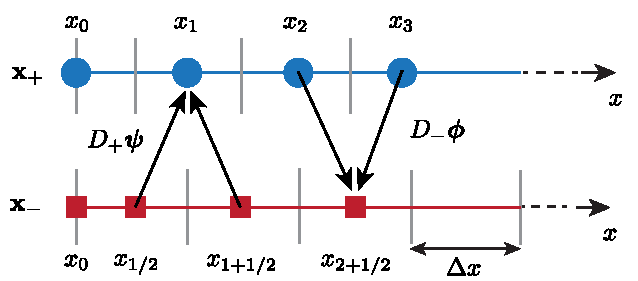
\includegraphics[width=\linewidth]{figures/difference_operators.pdf}
\caption{Example of second order difference approximations on staggered grids in one dimension.}
\label{fig:grids}
\end{figure}
              

%----------------------------------------------------------------------------------------

\end{column} % End of the first column

\begin{column}{\sepwid}\end{column} % Empty spacer column

\begin{column}{\twocolwid} % Begin a column which is two columns wide (column 2)

\begin{columns}[t,totalwidth=\twocolwid] % Split up the two columns wide column

\begin{column}{\onecolwid}\vspace{-.6in} % The first column within column 2 (column 2.1)

%----------------------------------------------------------------------------------------
%	MATERIALS
%----------------------------------------------------------------------------------------



%----------------------------------------------------------------------------------------

\end{column} % End of column 2.1

\begin{column}{\onecolwid}\vspace{-.6in} % The second column within column 2 (column 2.2)

%----------------------------------------------------------------------------------------
%	METHODS
%----------------------------------------------------------------------------------------


%----------------------------------------------------------------------------------------

\end{column} % End of column 2.2

\end{columns} % End of the split of column 2 - any content after this will now take up 2 columns width

%----------------------------------------------------------------------------------------
%	IMPORTANT RESULT
%----------------------------------------------------------------------------------------

\begin{alertblock}{Accuracy of free-surface boundary condition implementations in 1D}
  \begin{figure}
  \subfloat[time $T=10$]
  {\includegraphics[scale=1.4]{figures/rk4_sbp4_10}}
  \subfloat[time $T=100$]
  {\includegraphics[scale=1.4]{figures/rk4_sbp4_100}}
  \subfloat[time $T=10$]
  {\includegraphics[scale=1.4]{figures/rk4_sbp6_10}}
  \subfloat[time $T=100$]
  {\includegraphics[scale=1.4]{figures/rk4_sbp6_100}}
    \caption{Error as a function of simulation time at time $T$ (number of reflections) (a),(b) compares FS1 vs new fourth-order boundary
    implementations, (c), (d) compares FS1 vs new sixth-order boundary implementations}
  \end{figure}
  Test using initial condition $\sigma(x,0) = v(x,0) = e^{-a(x-0.5)^2}$ for $0 \leq x \leq 1$. Boundary conditions are:
  $\sigma(0,t) = \sigma(1,t) = 0$. We use $a = 100$, $\rho = \mu = 1$, and let the solution reflect against each boundary
  $T$ times per boundary. A fourth-order Runge-Kutta method with time step $\Delta t = 0.4\Delta x$ is used in time.
  SBP\textbf{X}\textbf{Y}, \textbf{X} = interior order of accuracy, \textbf{Y} = \textbf{W}eak or \textbf{S}trong enforcement of boundary conditions.
%  SBPW (weak enforcement of boundary conditions) and SBPS strong enforcement of boundary conditions. SBP4 is
%  fourth-order accurate (interior) and SBP6 is sixth-order accurate (interior).
            
\end{alertblock} 

%----------------------------------------------------------------------------------------

\begin{columns}[t,totalwidth=\twocolwid] % Split up the two columns wide column again

\begin{column}{\onecolwid} % The first column within column 2 (column 2.1)


 \begin{block}{The elastic wave equation with a weak enforcement of the free-surface boundary condition}
  Elastic wave equation (anti-plane) with velocity $v$ and shear stresses
    $\sigma = (\sigma_{13},\sigma_{23})^T$:
  \begin{align}
    \begin{aligned}
    \rho v_t &= \nabla \cdot \sigma, 
    \nonumber
    \
    \sigma_t = \mu\nabla v, \ (x,y) \in \Omega,
    \nonumber
    \\
    T &= \hat{n}^T\sigma = 0 \ \mbox{on}\ \Gamma.
    \end{aligned}
    \nonumber
  \end{align}

  Variational formulation with weak enforcement of boundary conditions:
  \begin{align}
    \begin{aligned}
    \int_{\Omega} \rho \phi v_t d\Omega = \int_{\Omega} \phi \nabla \cdot \sigma d\Omega - \int_{\Gamma}\phi
    (T-\hat{T})ds,
    \nonumber
    \\
    \int_{\Omega} \frac{1}{\mu}\varphi^T \sigma_t d\Omega = \int_{\Omega} \varphi^T \nabla v d\Omega - \int_{\Gamma}\varphi^T
    (v-\hat{v})\hat{n}ds.
    \end{aligned}
    \label{elastic_var}
  \end{align}
  Fluxes chosen as
  \begin{align}
    \hat{T} = 0, \ \hat{v} = v - ZT, Z = \rho \mu.
  \end{align}
  The choice $\phi = v$ and $\varphi = \sigma$ yields energy rate:
  \begin{align}
    \frac{1}{2}\frac{d}{dt}\int_{\Omega} \rho v^2 + \frac{1}{\mu}\sigma^T\sigma d\Omega = -\int_{\Gamma} ZT^2ds \leq 0. 
  \end{align}


\end{block}  

%----------------------------------------------------------------------------------------

\end{column} % End of column 2.1

\begin{column}{\onecolwid} % The second column within column 2 (column 2.2)

  \begin{block}{Provably stable and high-order accurate finite difference approximations}
    Variational formulation of elastic wave equation (\ref{elastic_var}) approximated by
    \begin{align}
      \phi^T\rho H_+ \frac{dv}{dt} &=\phi^T Q_+ \sigma -(r^T_+\phi)^T r^T_+(T-\hat{T}), 
      \nonumber
      \\
      \varphi^T\mu  H_- \frac{d\sigma}{dt} &=\varphi^T Q_- v -(r^T_-\varphi)^T r^T_+\hat{n}(v- \hat{v}), 
      \nonumber
    \end{align}
    where $D_- = P^{-1}Q_-$, $D_+ = P^{-1}Q_+$ (difference approximations, see Figure \ref{fig:grids}), $H = diag(..)$
    (quadrature rule), and vectors $r_-$, $r_+$ restricting solution to
    the boundary.

    The choice $\phi = v$, $\varphi = \sigma$ yields energy rate
    \begin{align}
      \begin{split}
      \frac{1}{2}\frac{d}{dt}(v^T\rho H_-v + \sigma^T\mu^{-1}H_+\sigma) = v^T(Q_+ + Q_-^T + \hat{n}r_+r_-^T)\sigma \\
      + \mbox{Diss}, 
    \end{split}
      \nonumber
    \end{align}
    where $\mbox{Diss} \leq 0.$ The scheme is a summation-by-parts (SBP) scheme if:
    \begin{align}
    Q_+ + Q_-^T + \hat{n}r_+r_-^T = 0.
    \label{SBP}
    \end{align}
    In 1-D FS1 satisfies (\ref{SBP}) with $\mbox{Diss} = 0$. Thus
      $dE_h/dt = 0.$


  \end{block}



%----------------------------------------------------------------------------------------

\end{column} % End of column 2.2

\end{columns} % End of the split of column 2

\end{column} % End of the second column

\begin{column}{\sepwid}\end{column} % Empty spacer column

\begin{column}{\onecolwid} % The third column

%----------------------------------------------------------------------------------------
%	CONCLUSION
%----------------------------------------------------------------------------------------
\begin{block}{Construction of free-surface boundary conditions} 
  We construct new difference approximations satisfying (\ref{SBP}). These approximations are the same as FS1 in the
  interior, but uses different boundary closures. These boundary closures incur a small increase in
  computational cost because of having more non-zero coefficients in the difference stencils near the boundary. On the
  other hand, we gain free parameters which are tuned to minimize the truncation error.
\end{block}

\begin{block}{Conclusions}
  The free-surface boundary condition at the Earth's surface give rise to surface waves which play a crucial role in
  ground motion estimation.  In this work we aim for improving the accuracy of
  the free-surface boundary condition by proposing new and provably stable implementations. Since our analysis is restricted to
  one dimension, we do not a priori know how the implementations perform in practical applications. However, our preliminary work in one dimension indicates that
  they can outperform the commonly used implementation (FS1) in most cases.
  The way these new implementations are designed also opens up the possibility for handling interface problems,
  which is essential in e.g., dynamic earthquake rupture simulations.

\end{block}

%----------------------------------------------------------------------------------------
%	ADDITIONAL INFORMATION
%----------------------------------------------------------------------------------------

\begin{block}{Additional Information}
  Our MATLAB demo implementation that was used to produce the results in this work is available here:
  \url{https://github.com/ooreilly/scec2016/}

\end{block}

%----------------------------------------------------------------------------------------
%	REFERENCES
%----------------------------------------------------------------------------------------

\begin{block}{References}
\nocite{*} 
\small{\bibliographystyle{unsrt}
\bibliography{references}\vspace{0.75in}}
\end{block}


%----------------------------------------------------------------------------------------

\end{column} % End of the third column

\end{columns} % End of all the columns in the poster

\end{frame} % End of the enclosing frame

\end{document}
